\documentclass[a4page]{article}

\usepackage{fullpage}
\usepackage{url}
\usepackage{acronym}
\usepackage{graphicx}

\author{Daniel Bischoff, Steffen Herrdum, Lin Xu}
\title{Exercise Plan}
\date{\today}

\begin{document}
\maketitle

\begin{table}[!th]
\begin{tabular}{l p{0.8\textwidth}}

Project Title: & Platform for Visualizing Life Cycle Assessment and Tracking of Consumer Products \\

\end{tabular}
\end{table}

\section{Introduction}
The quality of productions is getting harder being assessed, due to production procedure being allocated in global scope.
Without the information for instance, the resource of the food production remains unknown for the consumers.
It causes a huge production safety problem in the recent years.
This project is aiming at the tracking and tracing the productions Life cycle using simulated data to visualize and assess the Life period of productions. 

\section{Use Case Description}

Life Cycle Assessment\\
% DNL: Let's make this our main concern: (it is way easier to design a desktop app than to efficiently design a mobile layout)
A common use case would include a potential shopper who wants to gather information on the (type of) product he plans to buy.
The shopper is interested in sustainability, eco-friendliness, and labor conditions of the workers assembling the product.
He would like to view the origins of the product's components on a global scope map to develop a feeling for where the product and its components have been manufactured and how the long transportation distances affect the $\mathrm{CO}_2$-footprint of the product.
Furthermore, he would like to be provided with statistics and ratings concerning sustainability, $\mathrm{CO}_2$ emission of the manufacturers, etc.
It would be convenient to have all these influencing factors combined in a single rating.
An additional feature set could include specialized views for mobile devices where the user wants to have all the information at one glimpse.

\section{Platform, Libraries, and Framworks}
The target development platform for our Life Cycle Assessment (LCA) and tracking application is required to be Google Chrome. 
We aim at using the newest standardized contents of HTML5, CSS3, and JavaScript. We have to evaluate whether Firebase\footnote{https://www.firebase.com/} is suitable for our purposes as a back-end database provider.
Since our application requires visual representations of geographical maps we will use DataMaps\footnote{http://datamaps.github.io/} which is built on D3js\footnote{http://d3js.org/}.
Furthermore, we will directly use functionality provided by D3js to create visualizations of the product and component tracking data.

For user interface and layout we will use the Polymer\footnote{https://www.polymer-project.org/} framework. 
It provides easy ways of creating user interfaces based on principles of material design\footnote{https://www.google.com/design/spec/material-design/introduction.html} which we consider to be very appealing and simple.
We aim for simplicity in user interface design since we will make our application available on mobile browsers so that users can look up the \ac{LCA} and component tracking info while still at the store trying to decide which product to buy.

\section{Goals and Limitations}
The main goal of our application is to provide a fast and efficient way to look up \ac{LCA} data of products and their components.
Users should be able to search a certain product and get information on where the product and its components were assembled and which resources were used in what way.
The product life cycle will only be regarded as far as the product is acquired by its user.
We do not consider usage or disposal possibilities. 


We limit the scope of our application to use only constructed fictional data sets that we will try to make as generally applicable as possible. However, we will still limit the amount of products supported.

\section{Main Task}
The main problem in our application is the visual/graphical representation of very complex data in an easily understandable way.
Furthermore, we need to determine the structure of said data to be able to generalize and create more abstract relationships.
This is necessary to provide different layers in visualization resolution.
Finally we need to find ways to represent the data by using the previously mentioned frameworks.

\section{Milestones}

A detailed description of our timetable is illustrated in figure \ref{fig:gant-diagram}. We try to keep our timetable as tight as possible in order to have some additional time left for our \textit{Extra} features. Therefore we plan to finish the \textit{Prestudy} and \textit{Research} milestone during the first week and continue simultaneously with \textit{Modeling} concepts and a first \textit{Visualization Draft}. 

\begin{figure}[ht]
 \centering
 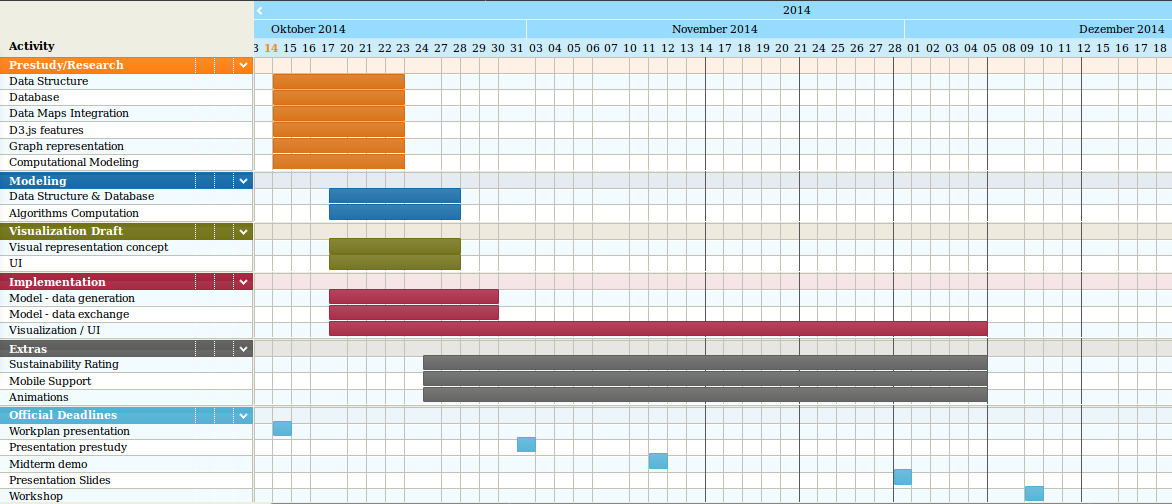
\includegraphics[scale=0.5]{gantt.png}
 \caption{Gantt diagram.}
 \label{fig:gant-diagram}
\end{figure}

%\newpage
%\section*{List of Abbreviations}
%\begin{acronym}
%\acro{LCA}{Life Cycle Assessment}
%\end{acronym}

\bibliographystyle{plain}
\bibliography{../reading/kernels,../reading/commute_time,diffusion,../reading/maths}

\end{document}

